% !TeX program = lualatex
% !TeX encoding = utf8
% !TeX spellcheck = uk_UA
% !BIB program = biber

\documentclass[]{beamer}
\usetheme{QuantumChemistry}
\usepackage{QuantumChemistry}
\usepackage{multirow}
\usepackage{makecell}
\usepackage{tabularray}


\graphicspath{{pictures/}}

\addbibresource{d:/Projects/LaTeX/QChem/Textbook2/QChemBook.bib}
\AtEveryCitekey{\clearfield{url}\clearfield{doi}}
\usetikzlibrary{chains, positioning}
\usepackage{ragged2e}
\usepackage{ifthen}

\newcommand\ddfrac[2]{\frac{\displaystyle #1}{\displaystyle #2}}

\newcommand\vertarrowbox[3][6ex]{%
  \begin{array}[t]{@{}c@{}} #2
  \left\uparrow\vcenter{\hrule height #1}\right.\kern-\nulldelimiterspace\\
  \makebox[0pt]{\scriptsize#3}
  \end{array}%
}
\usepackage{pdfpages}
\title[Лекції з квантової хімії]{\huge\bfseries Базисні набори}
\subtitle{Лекції з квантової хімії}
\author{Пономаренко С. М.}
\date{}
\let\vphi\varphi
\def\vxi{\vec{\xi}}
\begin{document}
%============================================================================
\usebackgroundtemplate{
	\tikz\node[opacity=0.15]{\includegraphics[width=\paperwidth,height=\paperheight]{background}};%
}
\begin{frame}
	\titlepage
\end{frame}
%============================================================================




%============================================================================
\begin{frame}[t]{Варіаційний принцип для обмеженого базису}{Варіаційний метод Рітца}
	Точна хвильова функція $\phi$ в загальному випадку \emphs{апроксимується} у вигляді \emphs{обмеженої лінійної комбінації} лінійно незалежних функцій (\emphs{які можуть бути і не ортонормованими}): $\chi_1$, $\chi_2$, $\ldots$ , $\chi_n$:
	\begin{equation}\label{eq:basis}
		\phi = \sum_{j = 1}^n c_j \chi_j,
	\end{equation}
	\begin{overprint}
		\onslide<1>
		коефіцієнти $c_j$ є параметрами, які визначаються шляхом мінімізації варіаційного інтеграла:
		\begin{equation}\label{key}
			W = \ddfrac{\int \phi^* \hat{H} \phi\, d\tau}{\int \phi^* \phi\, d\tau}.
		\end{equation}
		\onslide<2>
		\begin{multline*}\label{}
			\int \phi^* \hat{H} \phi\, d\tau = \int \sum_{j = 1}^n c_j^* \chi_j^* \hat{H} \sum_{k = 1}^n c_k \chi_k = \\ = \sum_{j = 1}^n c_j^* c_k \sum_{k = 1}^n \int \chi_j^* \hat{H} \chi_k\, d\tau = \sum_{j = 1}^n \sum_{k = 1}^n c_j^* c_k H_{jk}.
		\end{multline*}
		\onslide<3>
		\begin{multline*}\label{}
			\int \phi^*  \phi\, d\tau = \int \sum_{j = 1}^n c_j^* \chi_j^*  \sum_{k = 1}^n c_k \chi_k = \\ = \sum_{j = 1}^n c_j^* c_k \sum_{k = 1}^n \int \chi_j^*  \chi_k\, d\tau = \sum_{j = 1}^n \sum_{k = 1}^n c_j^* c_k S_{jk}.
		\end{multline*}
		де $S_{jk} = \int \chi_j^*  \chi_k\, d\tau $ --- інтеграли перекривання.
		\onslide<4>
		Інтеграл $W$
		\begin{equation}\label{}
			W = \ddfrac{\sum_{j = 1}^n \sum_{k = 1}^n c_j^* c_k H_{jk}}{\sum_{j = 1}^n \sum_{k = 1}^n c_j^* c_k S_{jk}}.
		\end{equation}
		є функцією від $n$ незалежних змінних $c_1$, $c_2$, $\ldots$, $c_n$:
		\begin{equation*}\label{}
			W = W(c_1, c_2, \ldots, c_n).
		\end{equation*}
		\onslide<5-7>
		\begin{onlyenv}<5>
			Умовою мінімуму у функції $W = W(c_1, c_2, \ldots, c_n)$ є:
			\begin{equation*}\label{}
				\frac{\partial W}{\partial c_i} = 0, \quad i = 1,2, \ldots, n,
			\end{equation*}

		\end{onlyenv}
		\begin{onlyenv}<5-6>
			Яка приводить до рівнянь, розв'язками яких є коефіцієнти $c_i$:
			\begin{equation}\label{eq:eq_c}
				\sum_{k = 1}^n (H_{ik} - S_{ik} W) c_k = 0, \quad i = 1,2, \ldots, n.
			\end{equation}
		\end{onlyenv}
		\noindent\only<6>{Отримана система лінійних однорідних рівнянь має \emphs{нетривіальні розв'язки} тільки тоді, коли її \emphs{детермінант дорівнює нулю}:}
		\begin{onlyenv}<6-7>
			\begin{equation}\label{}
				\mathrm{det}(H_{ij} - S_{ij}W) = 0.
			\end{equation}
		\end{onlyenv}
		\begin{onlyenv}<7>
			Розв'язком цього характеристичного рівняння знаходять $n$ коренів $W_1$, $W_2$, $\ldots$, $W_n$:
			\begin{equation*}
				W_1 \le W_2 \le \ldots \le W_n.
			\end{equation*}
			Найменше значення $W_1$ є оцінкою зверзу енергії основного стану, решта коренів в рамках варіаційного методу Рітца є оцінками зверху для енергії відповідних \emphs{збуджених станів}.

			%			Для знаходження хвильової функції основного стану необхідно найменший корінь рівняння підставити в систему рівнянь~\eqref{eq:eq_c} і знайти коефіцієнти $c_i$. Аналогічно знаходять хвильові функції збуджених станів.
		\end{onlyenv}
		\onslide<8>
		Включення додаткових функцій $\chi_k$ в \eqref{eq:basis} підвищує точність розрахованих значень енергій. Якщо функції $\{\chi_k\}$ у \eqref{eq:basis}  утворюють повний набір, то ми отримаємо \emphs{точні хвильові функції системи}.

		\medskip

		У квантовій хімії в якості базису можуть використовуватись мільйони доданків у \eqref{eq:basis} щоб отримати точні результати для молекул. Очевидно, для цієї роботи необхідний комп’ютер.

	\end{overprint}
\end{frame}
%============================================================================





%============================================================================
%\tikzstyle{every picture}+=[remember picture]
%\begin{frame}{Хвильові функції}
%	Шукати функції в загальному вигляді, а тим більше тривимірні ніхто не вміє. Однак, якщо ми приймемо припущення, що нам доступний якийсь \emphs{базисний набір} функцій $\chi_q$, то
%	\begin{equation*}\label{basis}
%		\phi_i(\vec{r}) = \sum\limits_{q=1}^{N_b}
%		\tikz[baseline]{
%			\node[fill=red!20,anchor=base] (t1){$c_{iq}$};
%
%		}
%		\tikz[baseline]{
%			\node[fill=cyan!20,anchor=base] (t2) {$\chi_q(\vec{r})$};
%		}
%	\end{equation*}
%	%    \begin{equation*}\label{}
%	%        \phi_i(\vec{r}) = \sum\limits_{q = 1}^{N_b} c_{iq}\chi_q(\vec{r}).
%	%    \end{equation*}
%	причому $\chi_q(\vec{r})$ \tikz\node [coordinate] (n2) {}; можуть бути неортогональними одна одній. При подібному фіксованому поданні задача пошуку форми орбіталей зводиться до пошуку $N_b$ коефіцієнтів представлення $c_{iq}$\tikz[na]\node [coordinate] (n1) {};, а це вже не так страшно, хоча б зрозуміло що робити.
%	\begin{tikzpicture}[>=latex,overlay]
%		\path[->](n1.north) edge [bend left] (t1.south);
%		\path[->] (n2.north west) edge [bend left] (t2.north);
%	\end{tikzpicture}
%\end{frame}
%============================================================================





%============================================================================
\begin{frame}{Побудова базисів}{}
	\begin{alertblock}{}\centering
		У квантової хімії є два основні підходи до побудови базисів.
	\end{alertblock}

	\begin{enumerate}\small
		\item \emphs{Метод молекулярних орбіталей (МО) як лінійна комбінація атомних орбіталей (АО) (скор. МО ЛКАО)}

		      \begin{block}{}\scriptsize\justifying
			      Його ідея полягає в наступному. Молекула -- це набір атомів. До великого об'єднання в молекулу, кожен атом мав свою електронну оболонку, в якій електрони жили собі на його особистих (атомних) орбіталях (АО). А потім прийшли інші атоми, і довелося електронам розподілитися якось по-новому. Але, інші атоми -- це по-суті збурення, а значить нові стани можуть бути схожі на старі, і значить в якості базису має сенс взяти стани електронів, які у них були до великого об'єднання атомів в молекулу. Очевидно, що цей хід думок більше черпає ідеї з образу сферичної молекули в вакуумі, тому він є основним саме для таких систем.
		      \end{block}

		\item \emphs{Плоскі хвилі}.

		      \begin{block}{}\scriptsize\justifying
			      Стани вільного електрона --- або так звані плоскі хвилі. Тому такий базис використовується в основному для кристалічних тіл. У ньому передбачається, що електрони рухається в нескінченній періодичній решітці, а атоми, до яких електрон притягається, це всього-лише збурення в його мандрах по кристалу.
		      \end{block}
	\end{enumerate}
\end{frame}
%============================================================================





%============================================================================
\begin{frame}{Базиси для МО ЛКАО}{Орбіталі слейтерівського типу (STO)}
	%----------------------------------------------------------------------------
	В якості базисних функцій для розрахунків використовують орбіталі слейтерівського типу  (STO), нормалізована форма яких має вигляд:
	\begin{equation*}
		\chi_s = \frac{(2\zeta_s)^{n + 1/2}}{[(2n)!]^{1/2}} r^{n - 1}e^{-\zeta_s r} \cdot Y_{lm}(\theta, \phi).
	\end{equation*}
	{\scriptsize \fullcite{Slater1930}}
	\begin{columns}
		\begin{column}{0.5\linewidth}
			\begin{center}
				\begin{tikzpicture}[]
					\begin{axis}[
							axis lines = middle,
							clip=false,
							ylabel={$\chi$},
							y label style={at={(axis description cs:-0.01,1)},anchor=east},
							xlabel={$r$}, x label style={at={(axis description cs:1,-0.01)},anchor=west},
							xmin=0, xmax=2.1,
							ymin=0, ymax=1.1,
							ticks=none,
							width = \linewidth,
							%y=1.7cm,
							%x=1cm,
						]

						\addplot[thick,
							domain=0:2, red, thick, samples=500,
						] {1*exp(-2*x)} node[black, pos=0.3,above,sloped] {$n = 1$};
						\addplot[thick,
							domain=0:2, blue, thick, samples=500,
						] {1*x*exp(-2*x)} node[black, pos=0.6,above,sloped] {$n = 2$};

					\end{axis}
				\end{tikzpicture}
			\end{center}
		\end{column}
		\begin{column}{0.5\linewidth}
			\begin{overprint}
				\onslide<1>
				Орбітальна експонента $\zeta$:
				\[\zeta = \frac{Z-\sigma}{n}\]
				де
				$Z$ --  заряд ядра,\\
				$\sigma$ -- константа екранування,\\
				$n$ -- ефективне квантове число.
				\onslide<2>
				Радіальні частини STO не мають вузлів і задовольняють асимптотичній поведінці точної хвильової функції поблизу ядра та на великих відстанях від нього. При $l = n - 1$ \texttt{STO} переходить в АО воднеподібного атома.
			\end{overprint}
		\end{column}
	\end{columns}
	%----------------------------------------------------------------------------
\end{frame}
%============================================================================



%============================================================================
\begin{frame}{Орбіталі гаусового типу (GTO)}\small
	%----------------------------------------------------------------------------
	\begin{block}{}\scriptsize
		Про базиси \fullcite[Глава 14, \S 14.1]{Sleta} або \fullcite[Chapter 15, 15.4]{Levine}
	\end{block}
	\begin{itemize}\small
		\item Для \emphs{атомних розрахунків} цілком достатньо використовувати в якості базисних функцій слейтерівські орбіталі (STO), параметри $\zeta$ цих орбіталей табульовані.

		      {\scriptsize [\fullcite{ClementiRoetti}]}

		\item При проведенні \emphs{молекулярних розрахунків}, взяття інтегралів (елементи матриці Фока, та матриці перекриття) із-за наявності фактора $e^{-\zeta r}$ становить математичні труднощі.

        \item В якості базисних функцій використовувати орбіталі, в яких замість фактора $e^{-\zeta r}$ вводиться $e^{-\alpha r^2}$, такі орбіталі називаються орбіталі гаусового типу GTO (gaussian-type orbitals).
	\end{itemize}
	\begin{block}{}\scriptsize\justifying
		[\fullcite{Boys}]
	\end{block}
	%----------------------------------------------------------------------------
\end{frame}
%============================================================================





%============================================================================
\tikzstyle{every picture}+=[remember picture]
\begin{frame}{Базисні функції 1s-STO та 1s-GTO}
	%----------------------------------------------------------------------------
	\(
	\underbrace{\tcbhighmath[drop fuzzy shadow, colframe=cyan]{\chi =  \left( \frac{\zeta}{\pi}\right)^{1^{}/2} e^{-\zeta r}}}_{ST\tikzmark{1}O}
	\)
	\hfill
	\(
	\underbrace{\tcbhighmath[drop fuzzy shadow]{g =  \left( \frac{2\alpha}{\pi}\right)^{3^{}/4} e^{-\alpha r^2}}}_{GT\tikzmark{2}O}
	\)

	\begin{center}
		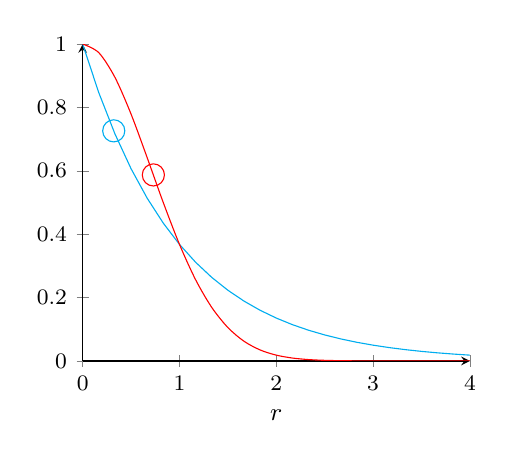
\begin{tikzpicture}[
				remember picture,
			]
			\begin{axis}[
					axis lines=left,
					xlabel=$r$,
					%ylabel=$\chi$,
					small,
				]

				\addplot [cyan, domain={0:4}]
				{1*exp(-x)} node [pos=0.1] (n1) {};


				\addplot [red, domain={0:4}, smooth]
				{1*exp(-x^2)} node [pos=0.2] (n2) {};

				%            \fill<1-> [cyan] (n1) circle (2pt);
				%            \fill<2-> [red]  (n2) circle (2pt);

			\end{axis}

			% for debugging purposes only
			\draw [cyan] (n1) circle (4pt);
			\draw [red]  (n2) circle (4pt);
		\end{tikzpicture}
	\end{center}

	\begin{tikzpicture}[
			remember picture,
			overlay,
			arrows={-Latex},
			ultra thick,
		]
		\draw[bend left=45, cyan] (n1) to (pic cs:1);
		\draw[bend right=45,red] (n2) to (pic cs:2);
	\end{tikzpicture}
	%----------------------------------------------------------------------------
\end{frame}
%============================================================================





%============================================================================
\begin{frame}{Загальний вигляд GTO}
    Орбіталі гаусового типу мають вигляд:
    \begin{equation*}\label{GTO}
        \tcbhighmath{%
            \mathrm{GTO}(x,y,z;\alpha,i,j,k) = \left(\frac{2\alpha}{\pi}\right)^{3/4}\sqrt{\frac{(8\alpha)^{i + j + k} i!j!k!}{(2i)!(2j)!(2k)!}} x^{i} y^{j} z^{k} e^{-\alpha r^2}
        }
    \end{equation*}

    \begin{itemize}
        \item при $i + j + k = 0$ (тобто, коли $i = 0$, $j = 0$, $k = 0$) GTO називаються $s$-типу;
        \item при $i + j + k = 1$ ми маємо GTO $p$-типу;
        \item при $i + j + k = 2$ ми маємо GTO $d$-типу;
        \item ...
    \end{itemize}

    \begin{block}{}\scriptsize\justifying
        Існує шість GTO $d$-типу, з множниками $x^2$, $y^2$, $z^2$, $xy$, $xz$ та $yz$. П’ять лінійних комбінацій (множники $xy$, $xz$, $yz$, $x^2 - y^2$ і $3z^2 - r^2$) можна утворити так, щоб вони мали однакову куту поведінка як п'ять реальних $3d$ AO; шоста комбінація з множником $x^2 + y^2 + z^2 = r^2$ подібна функції $3s$. Ця шоста комбінація часто опускається з базового набору.
    \end{block}

    %Notice that the difference between the STO and GTO is in the $r$-expotetnt The GTO squares the $r$ so that the product of the gaussian <<primitives>> (original gaussian equations) is another gaussian. By doing this, we have an equation we can work with and so the equation is much easier. However, the price we pay is loss of accuracy. To compensate for this loss, we find that the more gaussian equations we combine, the more accurate our equation.
    %
    %All basis set equations in the form STO-nG (where n represents the number of GTOs combined to approximate the STO) are considered to be <<minimal>> basis sets. The <<extended>> basis sets, then, are the ones that consider the higher orbitals of the molecule and account for size and shape of molecular charge distributions.
    %----------------------------------------------------------------------------
\end{frame}
%============================================================================





%============================================================================
\begin{frame}{Недоліки GTO. Контрактація базису}
	%----------------------------------------------------------------------------
	\begin{itemize}
		\item Поведінка GTO не схожа на справжню поведінка АО поблизу ядра, і швидко спадає на нескінченності (на відміну від STO).
		\item Якщо взяти достатню кількість GTO, можна апроксимувати STO.
	\end{itemize}

	\begin{equation*}
		\tcbhighmath[drop fuzzy shadow]{
			\mathrm{STO} \approx \mathrm{CGTO} =   \sum \mathrm{GTO} ,
		}
	\end{equation*}
	Набір GTO що апроксимують STO --- називається \emphs{стисненням}, або \emphs{контрактацією} (contractation) базису (CGTO --- contracted GTO's).

	\medskip

	\begin{block}{}\scriptsize\justifying
		Базиси  STO-NG, де $N$ --- число гаусових функцій (GTO), які \emphs{стискують} (\emphs{контрактують}) одну орбіталь STO називають \emphs{мінімальним базисом}. Під терміном \emphs{мінімальний базис} розуміють базисний набір, при якому \emphs{число базисних функцій атома визначається числом заповнених оболонок атома}.
		%    {\small Функції GTO називаються примітивними гаусовими функціями, або примітивами, і таких функцій потрібно істотно більше, ніж STO, але це з лишком компенсується аналітичними виразами для інтегралів.}
	\end{block}
	%----------------------------------------------------------------------------
\end{frame}
%============================================================================





%============================================================================
\begin{frame}{Приклад контрактації STO-3G}
	%----------------------------------------------------------------------------
	\begin{equation*}\footnotesize
		\text{STO-3G} =
		\highlight{cyan!50}{c_1 \cdot  \left(\frac{2\alpha_1}{\pi}\right)^{3/4}e^{-\alpha_1r^2}}{ge1}
		+
		\highlight{magenta!50}{%
		c_2 \cdot  \left(\frac{2\alpha_2}{\pi}\right)^{3/4}e^{-\alpha_2r^2}}{ge2}
		+
		\highlight{green!50}{%
		c_3 \cdot \left(\frac{2\alpha_3}{\pi}\right)^{3/4}e^{-\alpha_3r^2}}{ge3}
	\end{equation*}

	\begin{center}
		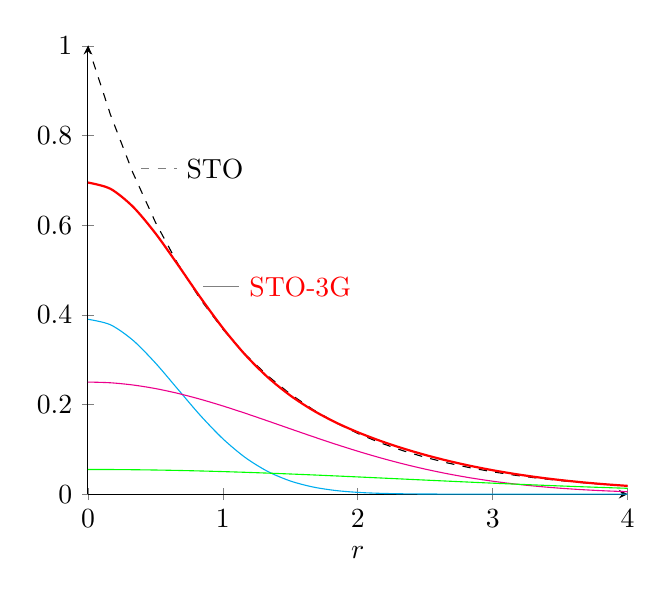
\begin{tikzpicture}[remember picture]
			\begin{axis}[
					axis lines=left,
					xlabel=$r$,
					%ylabel=$\psi$,
				]
				\newcommand{\es}{0.39*exp(-1.15*x^2)}
				\newcommand{\pe}{0.25*exp(-0.24*x^2)}
				\newcommand{\de}{0.055*exp(-0.09*x^2)}
				\addplot [dashed, domain={0:4}]
				{1*exp(-x)} node [pos=0.1, pin=0:STO] (s1) {};


				\addplot [cyan, domain={0:4}, smooth]
				{\es} node [pos=0.1] (g1) {};

				\addplot [magenta, domain={0:4}, smooth]
				{\pe} node [pos=0.2] (g2) {};

				\addplot [green, domain={0:4}, smooth]
				{\de} node [pos=0.2] (g3) {};

				\addplot [thick, domain={0:4}, smooth, red]
				{\es + \pe +\de} node [pos=0.2, pin=0:STO-3G] (gs) {};

			\end{axis}
		\end{tikzpicture}
	\end{center}

	\begin{tikzpicture}[
			%remember picture,
			overlay,
			arrows={-Latex},
		]
		%\draw<2>[]     (s1) to (pic cs:ge1);
		\draw[cyan] (g1) edge (ge1);
		\draw[magenta]  (g2) edge (ge2);
		\draw[green]  (g3) edge (ge3);
	\end{tikzpicture}
	%----------------------------------------------------------------------------
\end{frame}
%============================================================================





%============================================================================
\begin{frame}{Контрактація базисів}{}

	\begin{block}{}
		Для компактного опису базису використовують спеціальні позначення.
		Один з найбільш інформативних способів полягає в переліченні примітивних функцій і результатів їхньої контрактації.
	\end{block}

	\bigskip

	Запис
	\begin{equation*}
		(11s4p2d1f) \to [4s3p1d1f]
	\end{equation*}
	означає, що
	\begin{itemize}
		\item $11$ гаусових $s$-функцій утворює $4$ STO типу $s$,
		\item $4$ гаусові $р$-функції формують $3$ STO  типу $p$,
		\item $2$ гаусові $d$-функції утворюють одну STO типу $d$
		\item одна гаусова $f$-функція відповідає одній STO типу $f$.
	\end{itemize}

\end{frame}
%============================================================================





%============================================================================
\begin{frame}{Ієрархія базисів}{}
	\begin{enumerate}
		\item \emphs{Мінімальний базис}.
		      \begin{block}{}\scriptsize\justifying
			      Мінімальний базисний набір (minimal basis set) --- набір, в якому для кожного атома в молекулі використовується одна базисна функція для кожної орбіталі.
		      \end{block}
		\item \emphs{Розширені атомні базисні набори} --- кожну атомну орбіталь описують великою кількістю базисних функцій.
		      \begin{block}{}\scriptsize\justifying
			      Розрізняють двоекспоненційний (\emphs{Double Zeta}), триекспоненційний (\emphs{Triple Zeta}) базиси, тощо. Якщо розширення базису застосовується тільки до валентних орбіталей, базиси називаються \emphs{валентно-розщепленими}.
		      \end{block}
		\item \emphs{Поляризаційні функції}
		      \begin{block}{}\scriptsize\justifying
			      Застосовуються при описі хімічного зв'язку для врахування зміщення центру тяжіння електронного заряду, а також абсолютно необхідні для розрахунків з урахуванням кореляції електронів, щоб забезпечити опис збуджених станів.
		      \end{block}
		\item \emphs{Дифузні функції}.
		      \begin{block}{}\scriptsize\justifying
			      Вважливі для правильного опису аніонів та слабких зв'язків (наприклад, ван-дер-ваальсових та водневих зв'язків). Зазвичай це гауссіани $s$- і $p$-типу з малими експоненціальними множниками, що повільно спадають зі збільшенням відстані від ядра.
		      \end{block}
	\end{enumerate}
\end{frame}
%============================================================================





%============================================================================
\begin{frame}{Молекулярні базиси Попла}{}
	\begin{onlyenv}<1>
		Валентно-розщеплений базовий набір всіх атомів молекули:
		\begin{equation*}
			\tcbhighmath{
				\text{n-lmG},\quad
				\text{n-lmkG}
			}
		\end{equation*}
		\begin{itemize}
			\item $n$ --- задає число GTO для опису внутрішніх оболонок,
			\item Дві цифри $l$ та $m$ (або три $l$, $m$, та $k$) визначає число GTO, що входять до CGTO для валентних оболонок.

			      \medskip

			      {\small Кількість цифр $lm$ або $lmk$ вказують на валентний набір, що використовується --- Double Zeta або Triple Zeta. }
		\end{itemize}
        \vspace*{2em}
		\begin{equation*}
			\phi_i =
            \highlight{cyan!10!white}{
                c_{i1}\cdot
                \borderlight{cyan}{
                    \sum_r^n C_r g_r(\alpha_r)
                        }{c1}
                    }{g1} +
             \highlight{red!10!white}{
                 c_{i2} \cdot
                 \borderlight{red}{
                     \sum_s^l C_s g_s(\alpha_s)
                         }{c2} +
                 c_{i3} \cdot
                 \borderlight{red}{
                     \sum_t^m C_t g_t(\alpha_t)
                         }{c3}}{g2}
		\end{equation*}
    \begin{tikzpicture}[
        overlay,
        %			arrows={-Latex},
        sigd/.style = {anchor=north, font=\scriptsize},
        sigu/.style = {anchor=south, font=\scriptsize},
        ]
        \draw[->] (g1.south) to ++(-90:0.25cm) node[sigd] {Внутрішня оболонка};
        \draw[->] (g2.south) to ++(-90:0.25cm) node[sigd] {Валентна оболонка};
        \draw[->] (c1.north) to ++(90:0.25cm) node[sigu] {CGTO $\chi_1(\zeta_1)$};
        \draw[->] (c2.north) to ++(90:0.25cm) node[sigu] {CGTO $\chi_2^{\prime}(\zeta_2)$};
        \draw[->] (c3.north) to ++(90:0.25cm) node[sigu] {CGTO $\chi_2^{\prime\kern-1.25pt\prime}(\zeta_3)$};
    \end{tikzpicture}
	\end{onlyenv}
	\begin{onlyenv}<2>
        \begin{alertblock}{}\centering
            Хвильові функції атомів в молекулах деформуються! Для опису їх спотворень в атомні базисні набори включають додаткові функції !
        \end{alertblock}
		Основні включення в базисні набори розділяють на:
		\begin{itemize}
			\item  \emphs{поляризаційні функції} $d$-типу для неводневих атомів (позначається \emphs{n-lm*} або \emphs{n-lmkG*}) або $p$-функцій для атомів водню (\emphs{n-ijG**} та \emphs{n-lm**}).

%            \orbital{s} \orbital[phase=-]{s}
%            \orbital{p} \orbital[phase=-]{p}
%            \orbital{sp3} \orbital[phase=-]{sp3}

			\item \emphs{дифузні функції} $s$-типу  і трьох $p$-типу (позначається \emphs{n-lm+G} або \emphs{n-lmk+G}). Набори \emphs{n-lm++G} та \emphs{n-lmk++G} отримані з попередніх додавань для атома водню трьох дифузних GTO p-типу.

		\end{itemize}
	\end{onlyenv}
\end{frame}
%============================================================================




%============================================================================
\begin{frame}{Мінімальні базиси STO-nG}{}
	\begin{itemize}
		\item Мінімальний базис (або одноекспоненційний, Single Zeta) --- набір, в якому для кожного атома в молекулі використовується одна базисна функція для кожної орбіталі.

		      \begin{center}
			      \begin{tabular}{llc}
				      \toprule
				      \thead{Атом}       & \thead {Набір STO} & \thead{Число функцій} \\ \midrule
				      \ce{H}, \ce{He}    & $1s$               & 1                     \\
				      \ce{Li} -- \ce{Ne} & $1s2s2p$           & 5                     \\
				      \ce{Na} -- \ce{Ar} & $1s2s3s3p$         & 9                     \\ \bottomrule
			      \end{tabular}
		      \end{center}
		\item Для кожного з атомів від \ce{Na} до \ce{Ar} мінімальними AO є $1s$, $2s$, $2p_{x,y,z}$, $3s$, $3p_{x,y,z}$ (але не $3d$).
	\end{itemize}
\end{frame}
%============================================================================




%============================================================================
\begin{frame}{Поляризаційні функції\footnote{Включення до базисного набору поляризаційних функцій вказується літерою <<P>> або зірочкою <<*>>.}}{}
	\begin{itemize}
		\item Поляризаційні функції є базисними функціями із вищим кутовим моментом, наприклад, функції $p$-типу функції в атомі \ce{H} або $d$-типу для \ce{O}.
		\item Поляризаційні функції вносяться в набір, якщо розглядається поляризація атомів (в електричних полях, або в молекулах).
		      \begin{itemize}
			      \item Наприклад, дипольний момент \ce{H2O} становить $0.96$~$ea_0$ для базису 6-31G, і більш точне значення $0.83$~$ea_0$ для базису 6-31G*.
			      \item Іншим прикладом є бар'єр для обертання в \ce{H2O2}. Взаємодія між диполями вздовж полярних зв'язків \ce{OH} описується точніше завдяки поляризаційним функціям.
		      \end{itemize}
	\end{itemize}

\end{frame}
%============================================================================




%============================================================================
\begin{frame}{Дифузні функції\footnote{Включення дифузних функцій до базису позначається символом <<+>>}}{}
	\begin{itemize}\small
		\item В \emphs{аніонах}, наприклад, зайвий електрон дуже слабко зв'язаний з ядром, що
		      проявляється в низькій спорідненості з електроном і значною віддаленістю електронної густини від ядра. Тому, властивості аніонів погано відтворюються навіть з великими базовими наборами.

		\item Для усунення невідповідності з експериментом в базисний поляризаційний набір включають дифузні функції $s$ і $p$-типу з малими значеннями експоненціальних коефіцієнтів $\alpha$, що обумовлює \emphs{великий розмір і віддаленість цих функцій від ядра}.

	\end{itemize}


	\begin{center}\footnotesize
		\renewcommand\theadfont{\scriptsize}
		Результати розрахунку енергій депротонування (ккал/моль) деяких сполук:
		\begin{tabular}{|l|c|c|c|c|c|}
			\hline
			\thead{Реакція}             & \thead{STO-3G} & \thead{3-21G} & \thead{6-31G(d)} & \thead{6-31+G(d)} & \thead{Експеримент} \\ \hline
			\ce{CH4 $\to$ CH3^- + H^+}  & 560            & 453           & 457              & 435               & 426                 \\ \hline
			\ce{H2O $\to$ OH^- + H^+}   & 565            & 450           & 429              & 402               & 398                 \\ \hline
			\ce{H2O $\to$ OH^- + H^+}   & 602            & 432           & 409              & 374               & 376                 \\ \hline
			\ce{C2H2 $\to$ C2H^- + H^+} & 496            & 405           & 403              & 382               & 381                 \\ \hline
		\end{tabular}
	\end{center}
\end{frame}
%============================================================================





%============================================================================
\begin{frame}{Застосування базисів Попла}{}

	\begin{block}\justifying
		Базисні набори розроблені досить давно і на сьогодні забезпечують одержання результатів лише середнього рівня точності.
	\end{block}

	\begin{center}
		\begin{tblr}{
			colspec={|Q[l, valign=m, font=\scriptsize]|Q[c, valign=m,  font=\scriptsize]|Q[c, valign=m, font=\scriptsize]|X[j, font=\tiny, valign=m]|},
			row{1}={font=\scriptsize},
			%        row{2}={font=\scriptsize},
			%        row{2-Z}={font=\scriptsize},
			stretch=0.5,
			}
			\hline
			\SetCell[r=2]{c}{Базиси} & \SetCell[c=2]{c} Число базисних функцій &   & \SetCell[r=2]{c}{Опис}                                                                                     \\ \cline{2-3}
			                         & {Неводневі                                                                                                                                               \\ атоми} &  Водень  &                                                               \\ \hline
			STO-3G                   & 5                                       & 1 & Економічний з точки зору витрат часу та машинних ресурсів. Точність дуже низька. Для тестових розрахунків. \\ \hline
			3-21G                    & 9                                       & 2 & Точніше описує валентні орбіталі і системи без поляризації.                                                \\ \hline
			6-31G*  або  6-31G(d)    & 15                                      & 2 & Системи з анізотропією заряду                                                                              \\ \hline
			6-31G**  або 6-31G(d,p)  & 15                                      & 5 & Там де є водневий зв'язок                                                                                  \\ \hline
			6-31+G*  або 6-31+G(d)   & 19                                      & 2 & Молекули з неподіленими парами, молекулярні аніони, збуджені стани.                                        \\ \hline
			6-31+G** або 6-31+G(d,p) & 19                                      & 5 & Уточнення для попереднього базису                                                                          \\ \hline
		\end{tblr}
	\end{center}
\end{frame}
%============================================================================





%============================================================================
\begin{frame}[t]{Кореляційно-узгоджені базиси}{}
	\begin{equation*}
		\tcbhighmath{\text{сс-pV$x$Z},}
	\end{equation*}
	де $x$ – експоненціальність базису ($x=D$, $T$, $Q$, $5$, $6$, $7$, \ldots)
	\begin{itemize}\small
		\item набори спеціально розроблені для урахування електронної кореляції та їх використання рекомендується для високоточних квантовохімічних розрахунків.

		\item Поляризаційні функції включені до цих наборів за замовчуванням, їх не потрібно вказувати.

		\item Дифузні функції можуть бути додані вказівкою префікса \emphs{aug}.

		\item %
		      \begin{onlyenv}<1>
			      Набори дуже швидко збільшуються у розмірі при зростанні $x$.
			      Тому на звичайних робочих станціях розрахунки в цих базисах вищі за VQZ
			      можливі лише малих молекул. Одночасно точність розрахунку швидко
			      зростає і здебільшого базиси сс-VTZ і сс-pVQZ забезпечують
			      гарну згода структурних параметрів молекул з експериментом.
		      \end{onlyenv}

		      \begin{onlyenv}<2>
			      \begin{center}\footnotesize
				      Контрактація GTO для атомів першого ряду
				      \renewcommand{\arraystretch}{1.5}
				      \begin{tabular}{c|c|c|c}
					      cc-pVDZ    & cc-pVTZ       & cc-pVQZ         & cc-pVQ5Z          \\ \hline
					      $(9s4p1d)$ & $(10s5p2d1f)$ & $(12s6p3d2f1g)$ & $(14s9p4d3f2g1h)$ \\ \hline
					      $[3s2p1d]$ & $[4s3p2d1f]$  & $[5s4p3d2f1g]$  & $[6s5p4d3f2g1h]$  \\ \hline
					      14         & 30            & 55              & 91
				      \end{tabular}
			      \end{center}
		      \end{onlyenv}
	\end{itemize}
\end{frame}
%============================================================================





%============================================================================
\begin{frame}{Basis Set Exchange}{}
	Базисні набори та літературні посилання для них доступні на веб-сайті \href{https://www.basissetexchange.org/}{Basis Set Exchange}.
	\begin{center}
		\includegraphics[width=\linewidth]{BSE}
	\end{center}
\end{frame}
%============================================================================





%============================================================================
\begin{frame}[fragile]{Задавання базису в ORCA}{Базис 6-31+G**}\scriptsize
	\tikz[remember picture,overlay] \node[opacity=0.3,inner sep=0pt, anchor=north east] at (current page.north east){\includegraphics[width=3cm]{orca_logo}};

	{\scriptsize\color{blue}%
	\begin{verbatim}
%basis
 NewGTO He
    S   3
    1         0.3842163400E+02       0.4013973935E-01
    2         0.5778030000E+01       0.2612460970E+00
    3         0.1241774000E+01       0.7931846246E+00
    S   1
    1         0.2979640000E+00       1.0000000
    P   1
    1         0.1100000000E+01       1.0000000
  end
end
\end{verbatim}
	}
	\vspace*{-2em}
	\[
		\chi_{1s} =
		C_1 \left(\frac{2 \alpha_1}{\pi}\right)^{3/4} e^{-\alpha_1 r^2} +
		C_2 \left(\frac{2 \alpha_2}{\pi}\right)^{3/4} e^{-\alpha_2 r^2} +
		C_3 \left(\frac{2 \alpha_3}{\pi}\right)^{3/4} e^{-\alpha_3 r^2}.
	\]

	\[
		\chi_{2s} =
		C \left(\frac{2 \alpha}{\pi}\right)^{3/4} e^{-\alpha r^2}.
	\]

	\[
		\chi_{1p_{x,y,z}} =
		C \left(\frac{2 \alpha}{\pi}\right)^{3/4}\sqrt{4\alpha}\, (x,y,z)\, e^{-\alpha r^2}.
	\]

\end{frame}
%============================================================================

\end{document}
